\newcounter{count}
\newcommand\PoissonTitle{%
  \frametitle{\refstepcounter{count} Poisson/Laplace equation~\thecount}}
\resetcounteronoverlays{count}


\begin{frame}[fragile]
\PoissonTitle
\begin{itemize}
\item Poisson equation/ Laplace equation.
      \begin{fleqn}
      \begin{equation}
      -\frac{\partial^2 u}{\partial x^2} = \begin{cases} f\left(x\right) \qquad Poisson \ equation \\ 
      0 \qquad \qquad Laplace \ equation \end{cases} \qquad \forall x \in \left[0,L\right]
      \label{eq:poisson}
      \end{equation}
      \end{fleqn}

\item The boundary condition
\begin{fleqn}
      \begin{equation}
       T\left(x,0\right) = \begin{cases} g\left(x\right) \qquad Neumann \ BC \\ 
      const. \qquad Dirichlet \ BC \end{cases} \qquad \forall x \in \left[0,L\right]
      \end{equation}
      \end{fleqn}      
      
\end{itemize}
\end{frame}

\begin{frame}[fragile]
\PoissonTitle
\begin{itemize}
\item Poisson equation solution in one-dimension
\begin{figure}
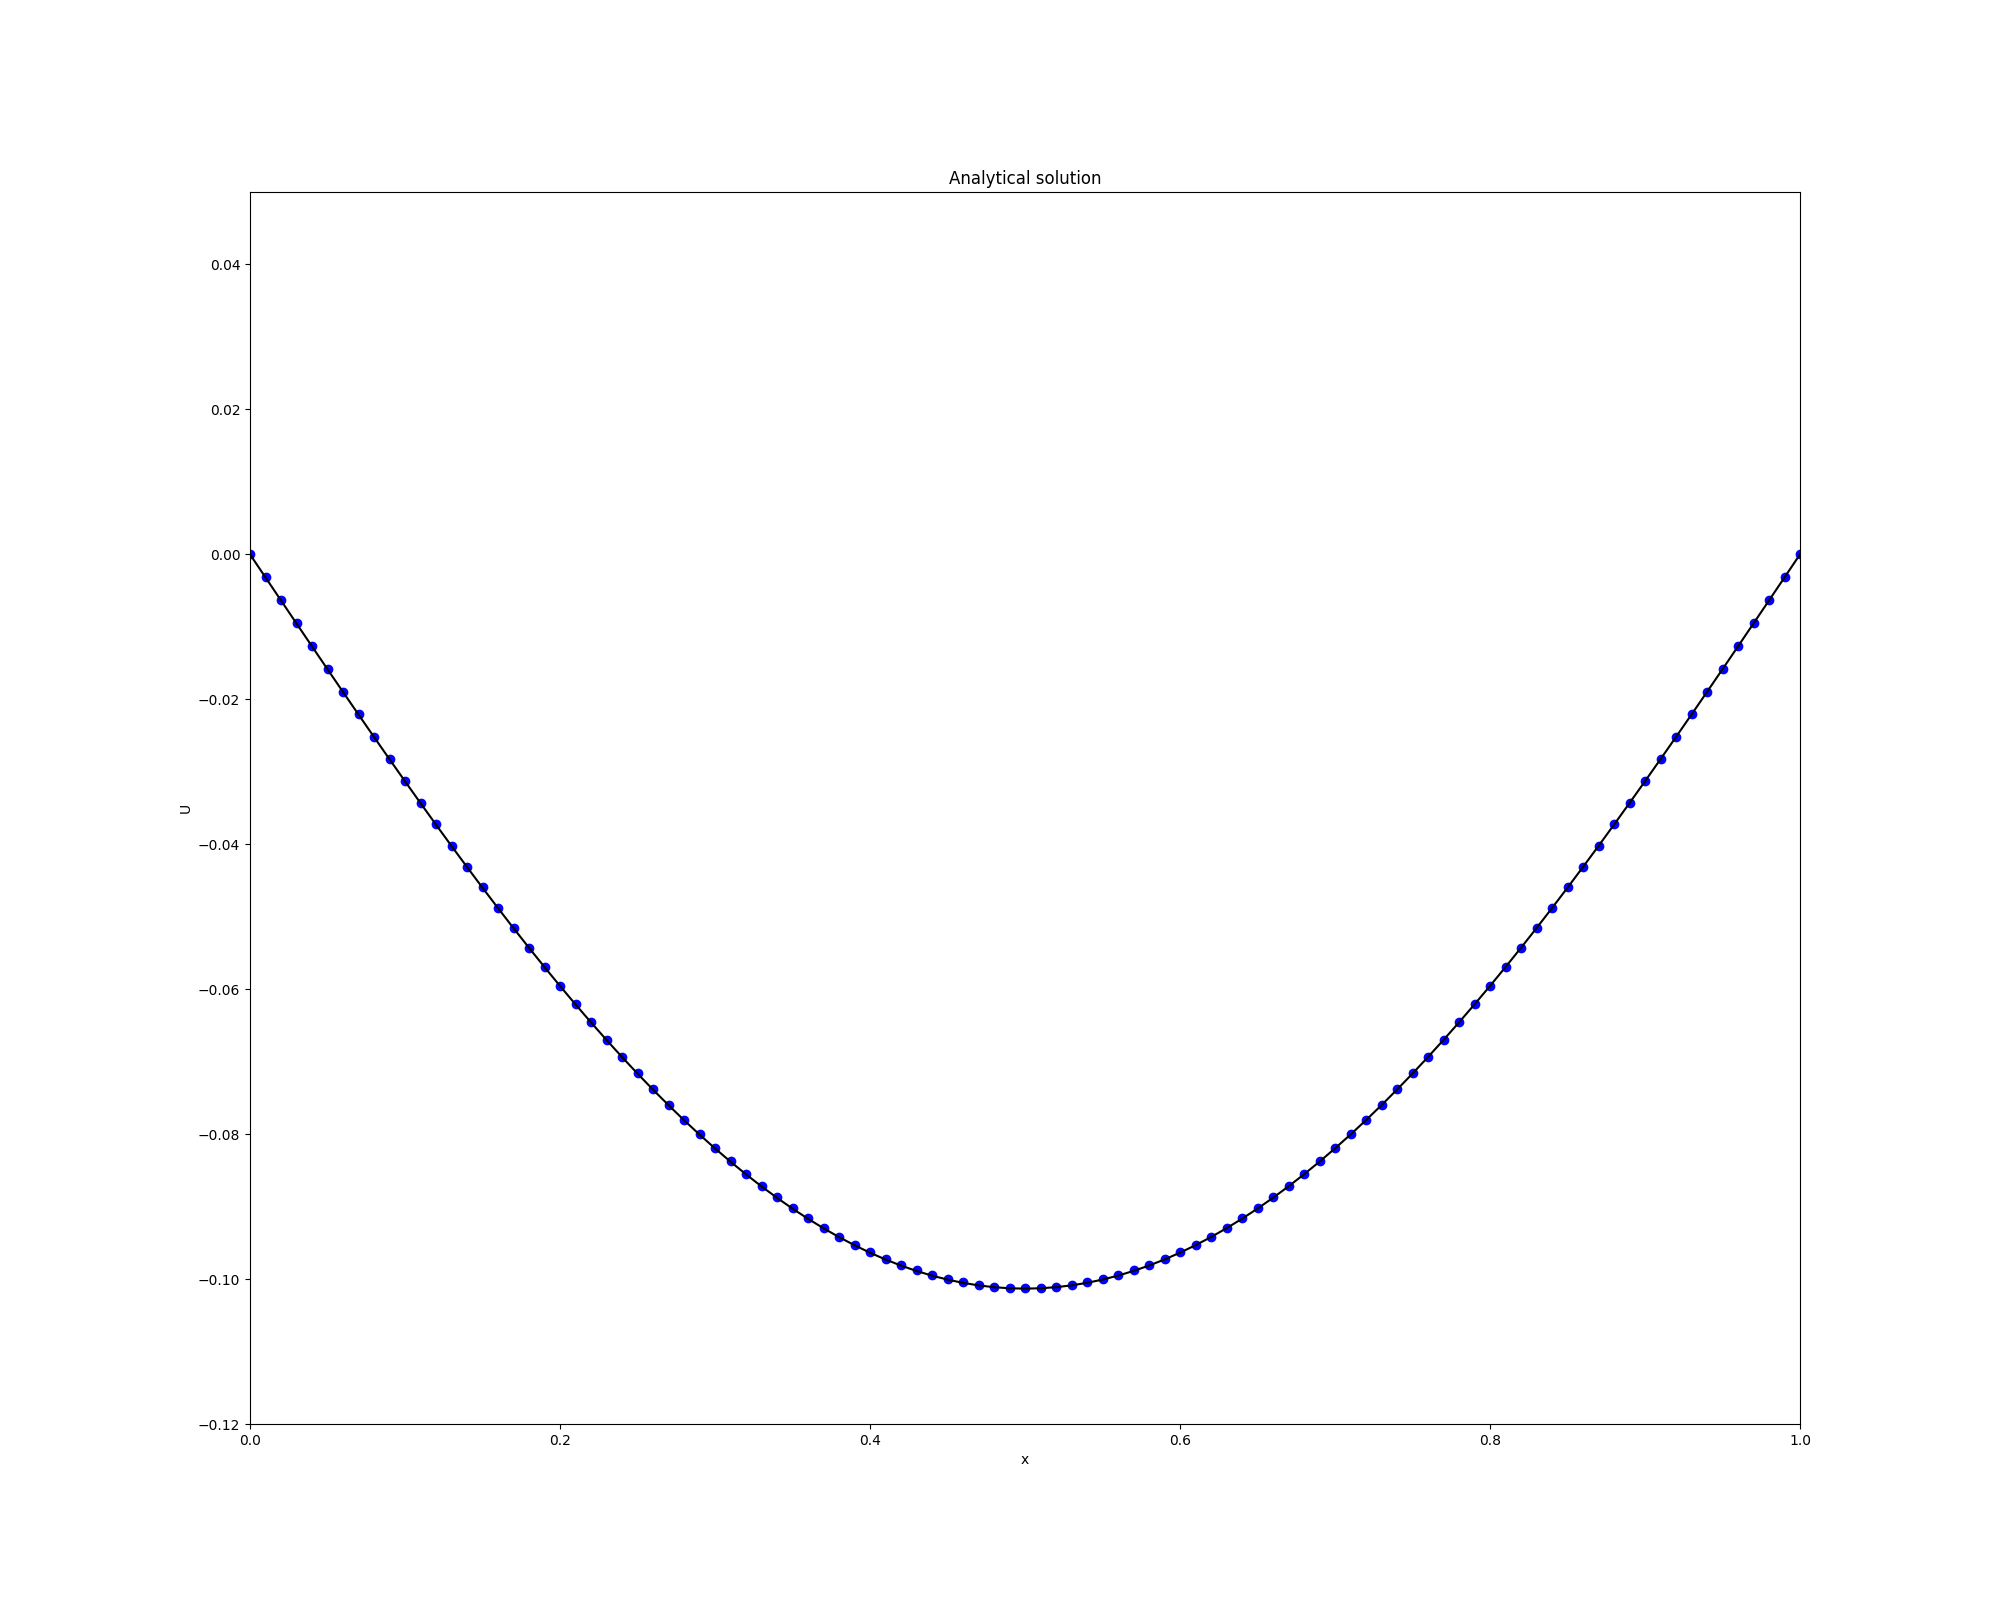
\includegraphics[width=\textwidth, height=0.4\textwidth]{./image/Poisson_analytical.png}%
%\includegraphics[width=0.5\textwidth, height=0.25\textwidth]{./image/%Poisson_final_steps.png}
\caption{Poisson equation solution}
\end{figure}
\end{itemize}
\end{frame}

\begin{frame}[fragile]
\PoissonTitle
\begin{itemize}
\item Sample of Poisson equation discretization in Python.
\lstinputlisting[language=Python, firstline=57, lastline=59]{./codes/Poisson1D.py}

\item The source term refers to $f\left(x\right)$

\end{itemize}
\end{frame}